% sec-proposedUI.tex
The proposed SimpleChef UI is designed around five main screens accessible via a bottom navigation bar: Home (Recipe Library), Calendar (Meal Planning), Add Recipe, Grocery List, and Profile. A global header with a back button appears on all sub-screens. The design follows a warm, appetizing color palette (primary: Sea Green \#2E8B57; accent: Sandy Yellow \#F4A261) and uses a legible sans-serif typography for clarity during cooking.

\textbf{Key Features:}
\begin{itemize}
  \item \textbf{Home Screen}: Responsive grid of recipe cards (2--3 columns) with hero images, titles, and badges (e.g., cook time, dietary tags). Search and filter by dietary restrictions, cook time, and difficulty.
  \item \textbf{Recipe Detail}: Scrollable view with hero image, key info strip (time, difficulty, servings, calories), expandable ingredients, and a prominent ``Begin Cooking'' button.
  \item \textbf{Step-by-Step Cooking Mode}: Fixed top bar with recipe name, step progress, and a timer dock showing stacked active timers. Each step displays a ``mise en place'' checklist of ingredients for that step, followed by instructions with embedded timer triggers. The bottom nav is replaced with cooking-specific controls (prev/next step, view all ingredients).
  \item \textbf{Calendar \& Meal Planning}: Monthly calendar with colored dots for planned days. Tapping a day reveals a bottom panel for adding meals from the library or quick-add foods, with daily calorie totals and optional statistics view.
  \item \textbf{Grocery List}: Auto-generated from meal plans, grouped by user-editable categories. Items are editable, draggable, and exportable via share sheet.
  \item \textbf{Add Recipe}: Input methods include paste text/URL, upload image, upload video, or manual entry. AI parsing populates structured fields; users verify and edit before saving.
  \item \textbf{Profile}: User info, calorie goals, dietary restrictions for filtering, and friends list for sharing recipes.
\end{itemize}

\textbf{Tools and Technology:}
\begin{itemize}
  \item \textbf{Frontend}: React Native (Expo) for cross-platform mobile development.
  \item \textbf{Backend}: FastAPI (Python) with PostgreSQL database.
  \item \textbf{Design}: Figma for wireframes and high-fidelity prototyping.
  \item \textbf{AI/ML}: For recipe parsing from text, image, or video inputs (to be integrated).
\end{itemize}

Figure~\ref{fig:SimpleChef_Wireframe} shows a wireframe of the main home screen layout, including the navigation bar and recipe grid.

\begin{figure}[ht]
  \centering
  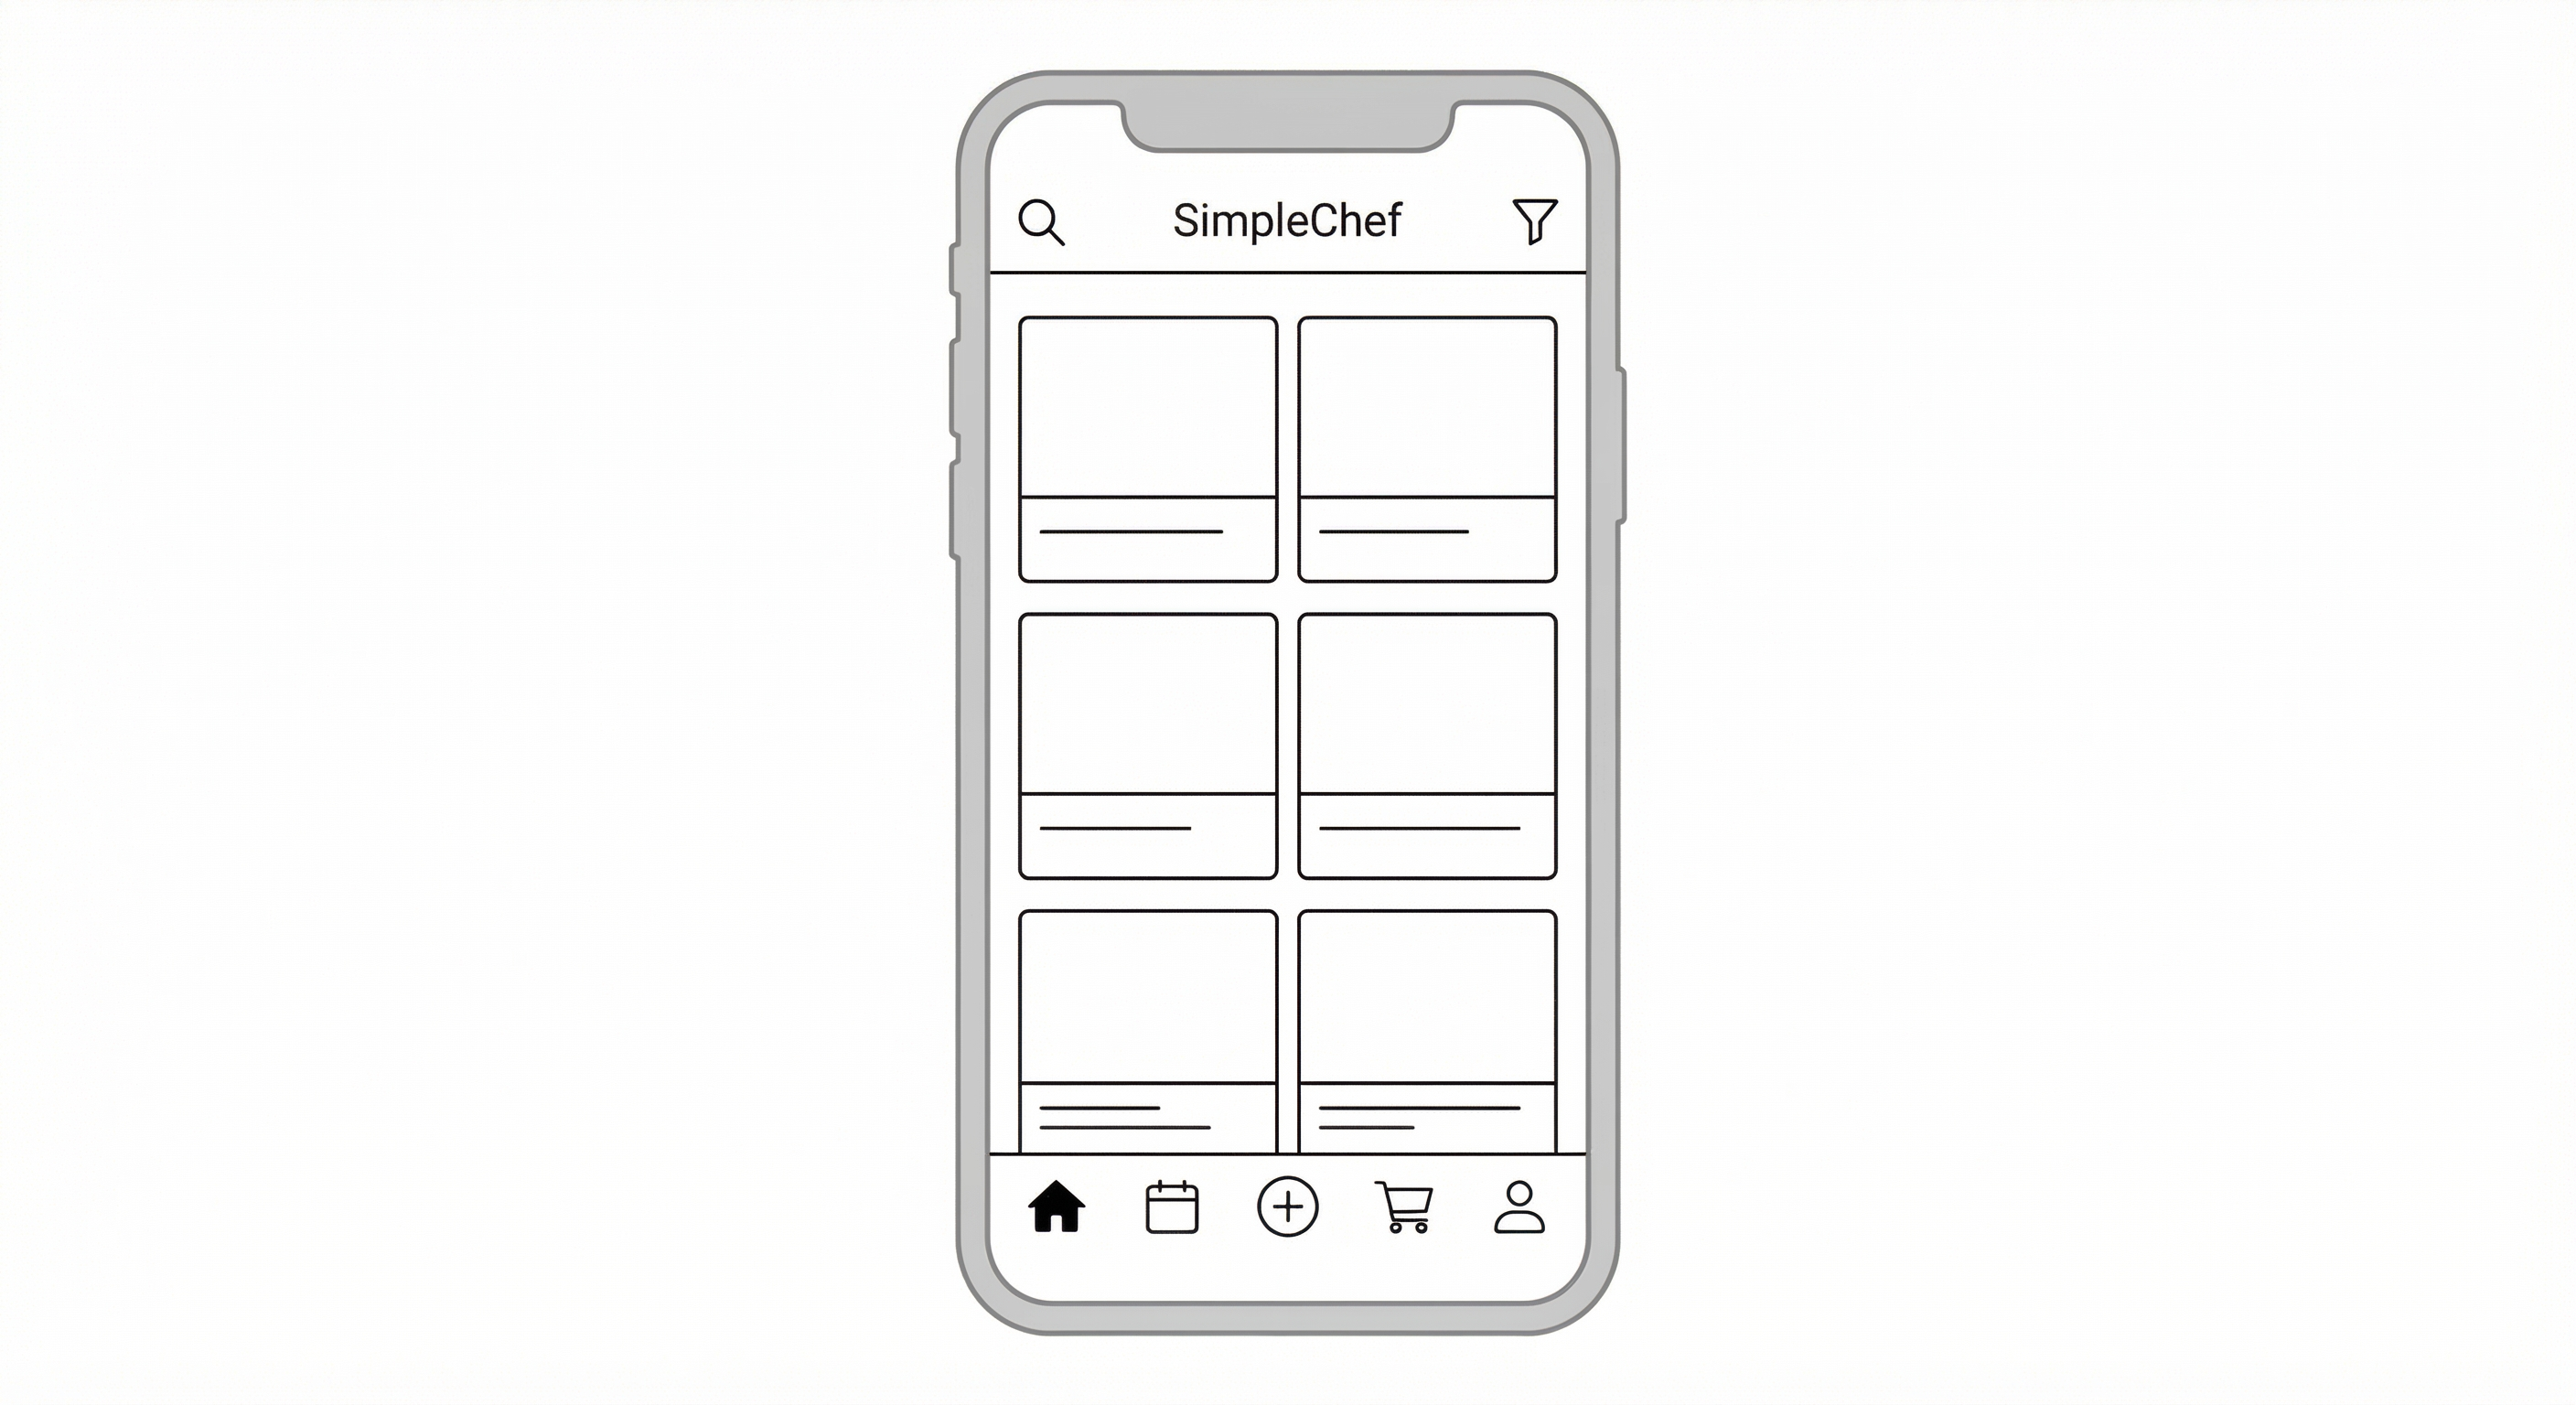
\includegraphics[width=\columnwidth]{figures/SimpleChef_Wireframe.png}
  \vspace{-10pt}
  \caption{Wireframe of the SimpleChef home screen (Recipe Library) with bottom navigation.}
  \label{fig:SimpleChef_Wireframe}
  \vspace{-10pt}
\end{figure}
